% Niveau :      PC
% Discipline :  Méca
% Mots clés :   Chaine, caténaire

\begin{exercise}{Les caténaires du TGV}{3}{Spé}
{Mécanique, Ondes mécaniques, Corde}{potier}

Le TGV (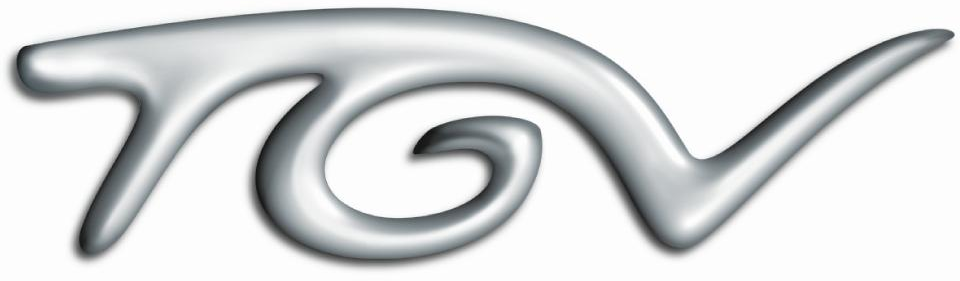
\includegraphics[height=1em]{meca/ondes_meca/TGV.png}) est alimenté en électricité par un pantographe (bras articulé) qui doit rester en contact avec la caténaire (le câble électrique d’alimentation) au cours du déplacement du train. Sur un ligne classique, ce câble est un câble de cuivre pur, tendu, dont la section vaut $150$  mm$^2$.

Montrer que quelles que soient les performances des moteurs électriques, la vitesse
du TGV est limitée par une limite physique qu’on évaluera.

On rappelle que le record actuel de vitesse du TGV est de $574,8$ km$\cdot$h$^{-1}$ en 2007.

Quelles solutions techniques à apporter pour augmenter cette vitesse limite sans que le 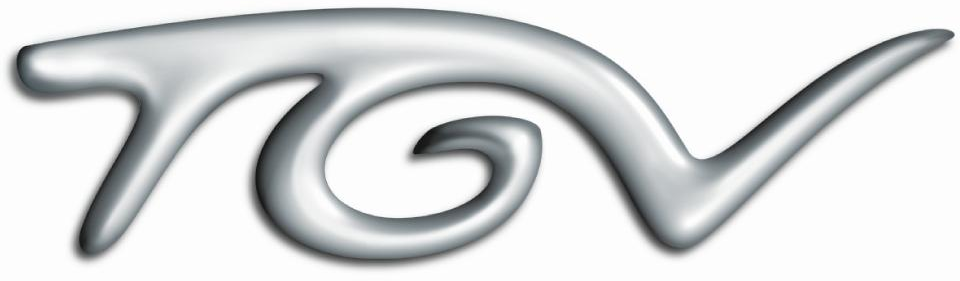
\includegraphics[height=1em]{meca/ondes_meca/TGV.png} ne se transforme en 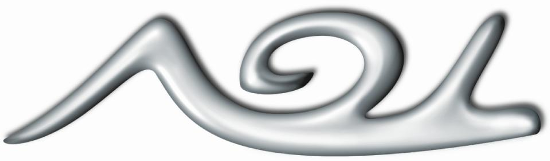
\includegraphics[height=1em]{meca/ondes_meca/GTV.png}...
\end{exercise}